% Appendix B

\chapter{Transformaciones de los datos} % Main appendix title

\label{AppendixB}

En este apéndice se detallan tres transformaciones del pipeline de datos presentado en la sección~\ref{sec:pipeline_datos}: el cálculo de la temperatura aparente, la corrección por pérdidas de la demanda regional y la depuración de la demanda horaria.

%----------------------------------------------------------------------------------------
\section{Cálculo de la temperatura aparente}
\label{sec:apendice_temp_aparente}
%----------------------------------------------------------------------------------------

La temperatura aparente se calcula según la formulación de Steadman \cite{steadman1994apparent}, con las adaptaciones de la implementación de Open-Meteo \cite{openMeteoCodigo}, que se expresan en la ecuación \ref{eq:temp_aparente}:

\begin{equation}
	AT = T + 0{,}348\,e - 0{,}70\,v_2 + 0{,}70\,\frac{Q}{v_2 + 10} - 4{,}25
	\label{eq:temp_aparente}
\end{equation}

\noindent donde \(T\) es la temperatura del aire en \textdegree C, \(e\) es la presión de vapor en hPa, \(v_2\) es la velocidad del viento a 2~m de altura en m/s y \(Q\) es la radiación absorbida. Estas tres magnitudes se obtienen según las ecuaciones \ref{eq:presion_vapor}, \ref{eq:viento_2m} y \ref{eq:radiacion_absorbida}:

\begin{equation}
	e = \frac{HR}{100}\; 6{,}105\, \exp\!\left(\frac{17{,}27\, T}{237{,}7 + T}\right)
	\label{eq:presion_vapor}
\end{equation}

\begin{equation}
	v_2 = 0{,}75\, v_{10}
	\label{eq:viento_2m}
\end{equation}

\begin{equation}
	Q = \max\left(0;\ 0{,}1\,(G - 550)\right)
	\label{eq:radiacion_absorbida}
\end{equation}

\noindent donde \(HR\) es la humedad relativa en porcentaje, \(v_{10}\) es la velocidad del viento a 10~m de altura en m/s y \(G\) es la radiación solar global en W/m\textsuperscript{2}.

%----------------------------------------------------------------------------------------
\section{Corrección por pérdidas de la demanda regional}
\label{sec:apendice_perdidas}
%----------------------------------------------------------------------------------------

La demanda de cada región se calcula a partir de su generación y de los intercambios con las regiones vinculadas, medidos en el SOTR. En términos formales, sea \(G_r\) la generación de la región \(r\), \(\mathcal{N}_r\) el conjunto de regiones vinculadas y \(F_{r\rightarrow j}\) y \(F_{j\rightarrow r}\) las mediciones del intercambio en ambos extremos del corredor. La demanda regional se calcula según la ecuación \ref{eq:demanda_regional}:

\begin{equation}
	D_r =
	G_r -
	\sum_{j \in \mathcal{N}_r}
	\frac{F_{r\rightarrow j}-F_{j\rightarrow r}}{2}
	\label{eq:demanda_regional}
\end{equation}

\noindent donde los intercambios son positivos cuando representan una exportación desde la región \(r\). La semidiferencia entre las mediciones de ambos extremos permite repartir las pérdidas del corredor en partes iguales entre las regiones vinculadas.

La figura \ref{fig:regiones_electricas_sotr}, tomada del SOTR, muestra el estado de generación e intercambio entre algunas regiones para un instante determinado.

\begin{figure}[H]
	\centering
	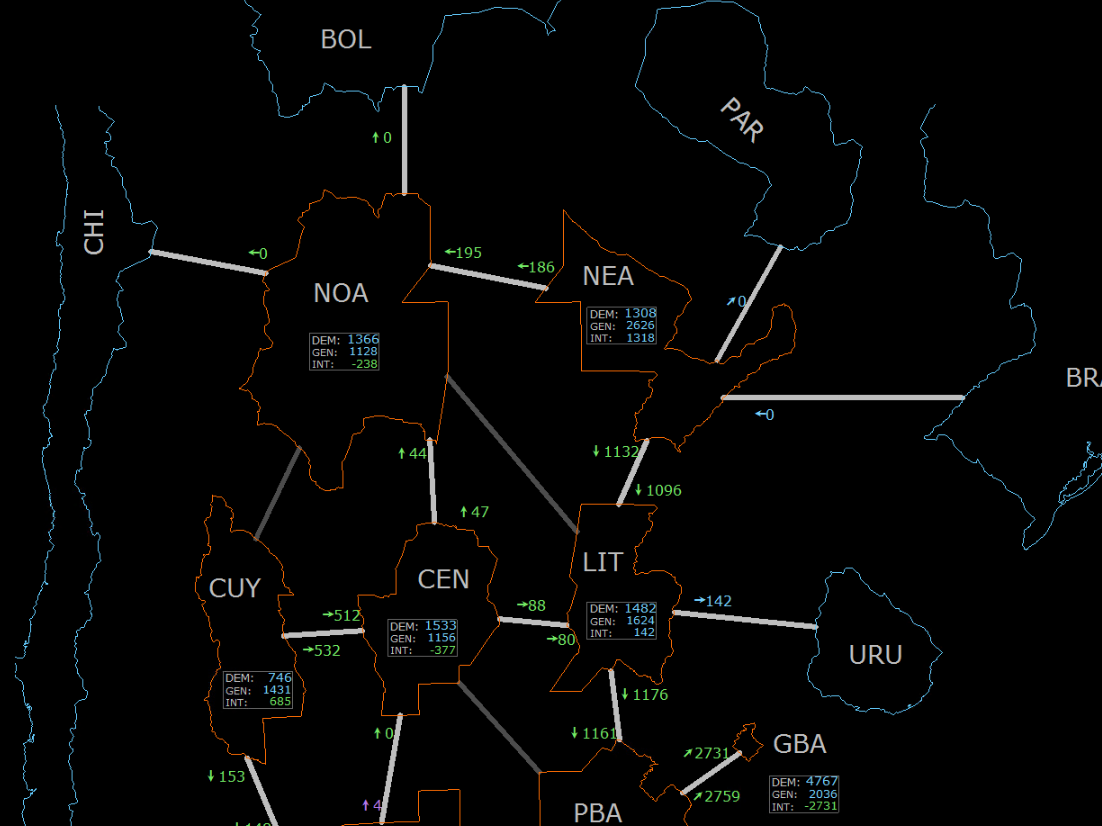
\includegraphics[width=\textwidth]{./Figures/regiones_electricas_sotr.png}
	\caption{Generación e intercambios entre regiones. Imagen del SOTR de CAMMESA para un instante determinado.}
	\label{fig:regiones_electricas_sotr}
\end{figure}

A modo de ejemplo, la demanda de LIT corregida por pérdidas para el instante de la figura se calcula según la ecuación \ref{eq:demanda_lit}. El intercambio con Uruguay es igual en ambos extremos, ya que corresponde a un vínculo interno de la central Salto Grande.

\begin{equation}
	\begin{aligned}
		D_{\mathrm{LIT}}
		={}& 1624
		-\left[
		\frac{-1096-1132}{2}
		+\frac{-80-88}{2}
		\right. \\
		&\left.
		+\frac{142-(-142)}{2}
		+\frac{1176-(-1161)}{2}
		\right]
	\end{aligned}
	\label{eq:demanda_lit}
\end{equation}

Al resolver las operaciones, resulta:

\begin{equation}
	D_{\mathrm{LIT}}
	=
	1624-
	\left(-1114-84+142+1168{,}5\right)
	=
	1511{,}5~\mathrm{MW}
\end{equation}

El valor obtenido, de 1511,5~MW, difiere de los 1482~MW que resultan sin considerar las pérdidas. En caso de no aplicar esta corrección, la demanda nacional agregada presentaría un error considerable introducido en los datos de entrenamiento de los modelos.

La implementación de esta corrección requirió definir todos los intercambios entre regiones y consultar una cantidad de medidores del SOTR sustancialmente mayor que si se hubiesen podido utilizar los medidores de demanda existentes.

%----------------------------------------------------------------------------------------
\section{Depuración de la demanda horaria}
\label{sec:apendice_depuracion}
%----------------------------------------------------------------------------------------

En la primera etapa de la limpieza se identifican valores extremos por región mediante el rango intercuartílico. Los límites se establecen a partir del primer y tercer cuartil y un factor de tres veces el rango intercuartílico. Los valores que quedan fuera de esos límites se reemplazan temporalmente por valores nulos y se estiman mediante interpolación lineal en el eje temporal. En la figura \ref{fig:correccion_outliers} puede verse un caso de corrección de valores extremos.

\begin{figure}[H]
	\centering
	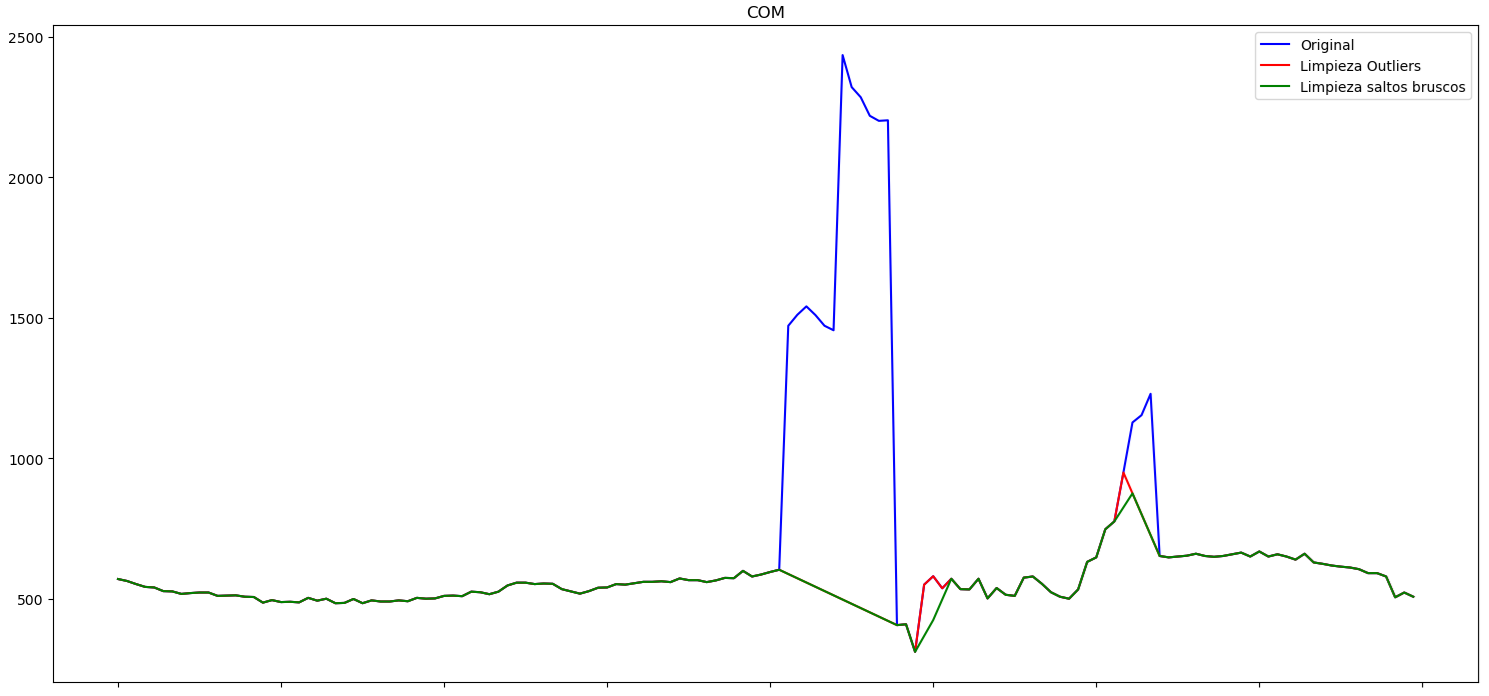
\includegraphics[width=\textwidth]{./Figures/correccion_outliers.png}
	\caption{Corrección de valores extremos.}
	\label{fig:correccion_outliers}
\end{figure}

El método de eliminación de outliers es eficiente para fallas de medición, donde se alcanzan valores extremos durante intervalos breves. Las correcciones más desafiantes son aquellas que corresponden a fallas reales del sistema eléctrico, por ejemplo, la desconexión intempestiva de una línea de transmisión que hace caer la demanda abruptamente. En estos casos, es deseable inferir el valor de demanda que se habría registrado sin la falla, ya que, a los fines del entrenamiento de un modelo predictivo, esa caída representa un error que debe desestimarse.

Por este motivo, en la segunda etapa se detectan escalones abruptos dentro de un mismo día. Un cambio se considera candidato a corrección cuando supera simultáneamente un umbral relativo del 7\,\% y un umbral absoluto de 100~MW. Estos valores fueron determinados a partir de la recomendación de los especialistas de CAMMESA en combinación con el análisis de amplios rangos temporales. La detección y corrección se ejecuta de manera iterativa, con un máximo de diez iteraciones. Los puntos identificados se interpolan y, cuando la interpolación no resulta posible en los extremos, se completan mediante propagación hacia adelante o hacia atrás. En la figura \ref{fig:correccion_saltos_bruscos} puede verse un caso de corrección de saltos bruscos.

\begin{figure}[H]
	\centering
	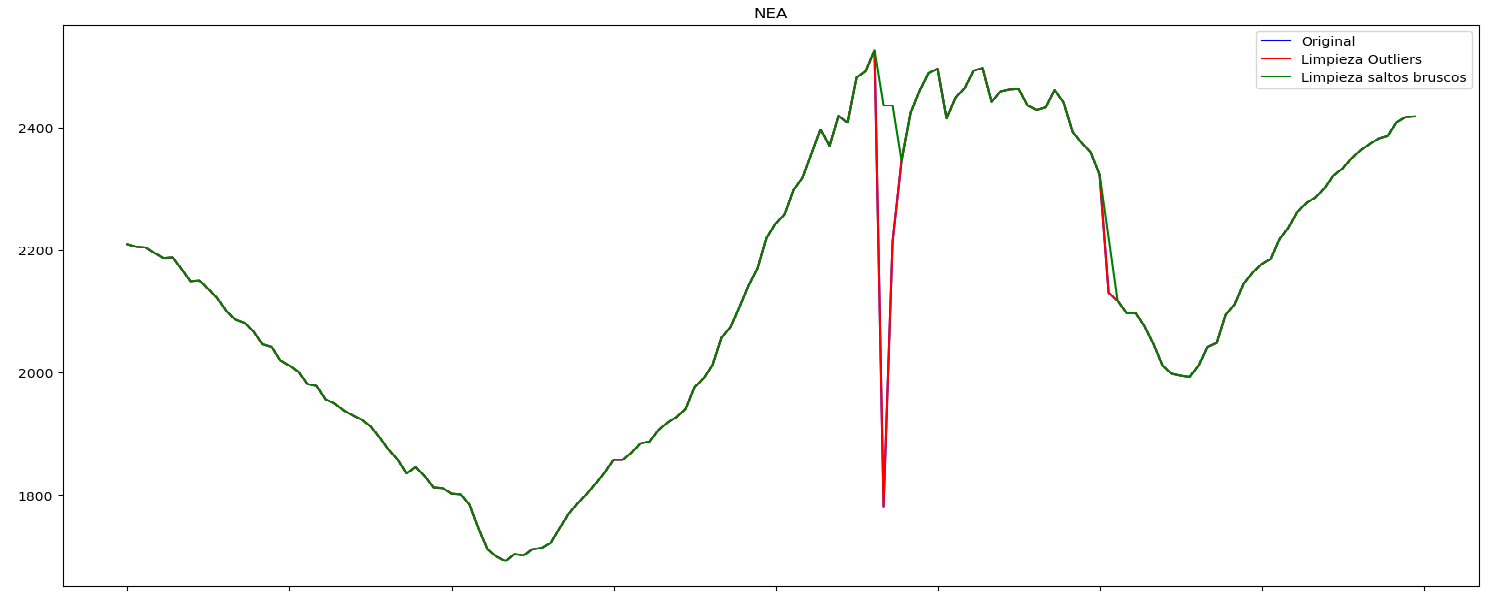
\includegraphics[width=\textwidth]{./Figures/correccion_saltos_bruscos.png}
	\caption{Corrección de saltos bruscos.}
	\label{fig:correccion_saltos_bruscos}
\end{figure}
